\subsection[Scenariusz (Kacper Połom)]{Scenariusz}
Test polega na zdalnym przesłaniu ładunku do urządzenia wykonującego, który symuluje pracę użytkownika.
\subsubsection[Aktorzy]{Aktorzy}
\begin{itemize}
    \item Tester - osoba przeprowadzająca test bezpieczeństwa systemu komputerowego za pomocą dedykowanego systemu
    \item Serwer - centralny punkt infrastruktury, który opowiada na zapytanie od testowanego systemu
    \item Urządzenie wykonujące - niewielkie urządzenie oparte o platformę Raspberry Pi Zero W, podłączone za pomocą portu USB do testowanego systemu
    \item Testowany system
\end{itemize}
\subsubsection[Założenia początkowe]{Założenia początkowe}
Uruchomiono testowany system
\subsubsection[Przebieg]{Przebieg}
Tester wpina urządzenie wykonujące przez port USB do testowanego systemu. urządzenie wykonujące zostaje zainstalowane jako klawiatura. Po poprawnym zainstalowaniu uruchamiany jest skrypt, który odpowiada za komunikację z serwerem i otrzymanie wymaganego ładunku do wykonania w testowanym systemie. Serwer potrafi rozróżnić testowane systemy na podstawie adresu IP, dzięki czemu wiele systemów może być testowanych w tym samym czasie. Tester przygotowuje zestaw znaków i skrótów klawiszowych, który zostanie wprowadzony do testowanego systemu. Rezultatem takiego działania może być wywołanie dowolnego programu zainstalowanego w testowanym systemie (np. wiersza poleceń) i wykorzystanie go do zdalnego wykonania kodu.
\begin{figure}[H]
    \centering
    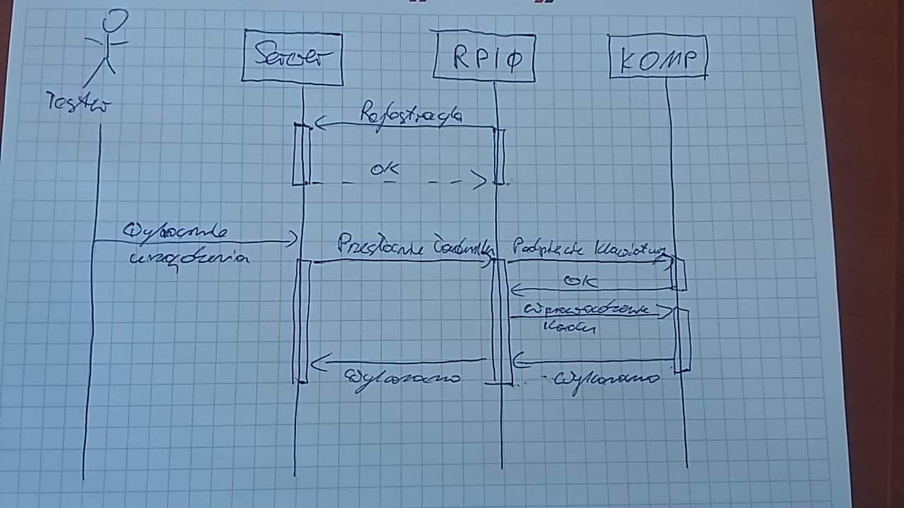
\includegraphics[width=\textwidth]{kp02}
    \caption{Placeholder}
    \label{fig:klawiatura}
\end{figure}